\chapter{Introduction}
The game of Go has challenged players around the world for centuries, and since the 1970's, international competitions have sought the world's best Go minds \cite{go}. The relatively simple rules of the game betray its true complexity and myriad moves; for example, there are 361 possible opening moves while chess has a mere 20 \cite{brit_go}. In fact, for the 19x19 Go board, about $\num{2e170}$ possible board states exist which is about $10^{90}$ times more than the number of atoms in the known universe \cite{go_num}. To produce a Go-playing artificial intelligence (AI) at the level of a human expert has been somewhat of a holy grail for machine learning researchers \cite{brit_go2}. Until 2014, the very best Go programs were only capable of occasionally beating top amateur players. However, in 2015, AlphaGo grabbed the world's attention with a landmark win, beating European champion Go player Fan Hui in a 5--0 upset \cite{brit_go3}. In March 2016, AlphaGo defeated 18-time world champion Lee Sedol 4--1. The success of AlphaGo's algorithms along with other research from DeepMind paved the way for improvements in reinforcement learning, especially in the previously intractable area of continuous control \cite{Mnih_2015}\cite{silver_2017}.

 Reinforcement learning (RL), the branch of machine learning concerned with how an actor should take actions in an environment to receive the most reward, has previously struggled with environments containing large state and/or action spaces. The recent  development of deep Q-network (DQN), deep policy gradients (DPG), and deep deterministic policy gradients (DDPG) within the past four years has opened the door to RL application in continuously controlled robotics  \cite{Mnih_2015}\cite{silver_lever_heess_degris_wierstra_riedmiller}\cite{lillicrap_2016}. This thesis covers the implementation of the off-policy, model-free DDPG algorithm in a purpose-built robot entered in the 2018 Cal Poly Roborodentia \cite{roborodentia}. Without knowledge of sensors or environment, the robot learns to control four independent mecanum wheels to move the robot to a desired position and orientation. 
 
 The paper is broken down into four chapters covering the various areas of development: mechanical, electrical, firmware, and reinforcement learning. Additionally, all project files can be found at \url{https://www.github.com/okayjustin/roborodentia2017}.


\section{Cal Poly Roborodentia}
The robot is designed to compete in the 2018 Cal Poly Roborodentia, the university's annual intramural robotics competition, and thus conforms to its particular specifications and requirements \cite{roborodentia}. Briefly, competitors must produce autonomous robots to collect and fire Nerf Rival Balls \cite{hasbro_2018}, shown in Figure \ref{fig:nerf_rival_balls}, into nets to win points. A drawing of the field is shown in Figure \ref{fig:roborodentia_field}. Two robots compete separately in each half so the effective field is a 4' wide by 8' long area enclosed by 4" walls. 1 inch PVC tubes along the 4' walls hold the balls which the robots fire into rectangular nets located along the 8' walls. The rules provide additional restrictions on robot dimensions, capabilities, and other aspects, to be covered in the following chapters.
\begin{figure}[H]   % [h] means here
	\centering 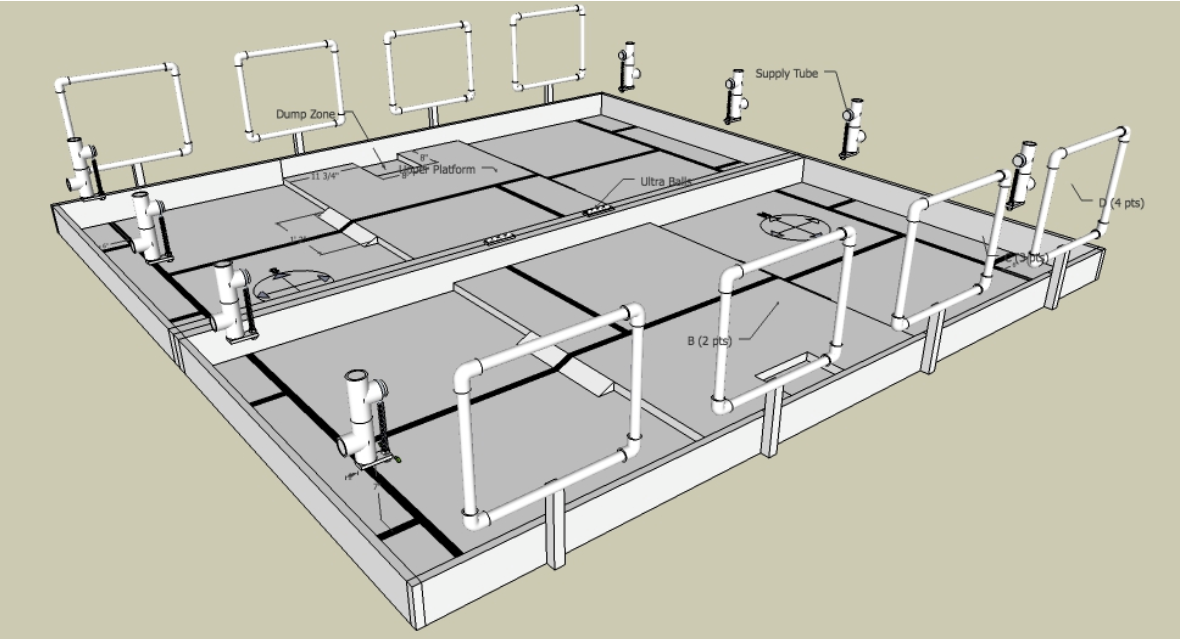
\includegraphics[width=6in, height=3.85in, keepaspectratio]{figures/roborodentia_field.png}
	\caption{Roborodentia Field \cite{roborodentia}}	\label{fig:roborodentia_field}
\end{figure}
\begin{figure}[H]   % [h] means here
	\centering 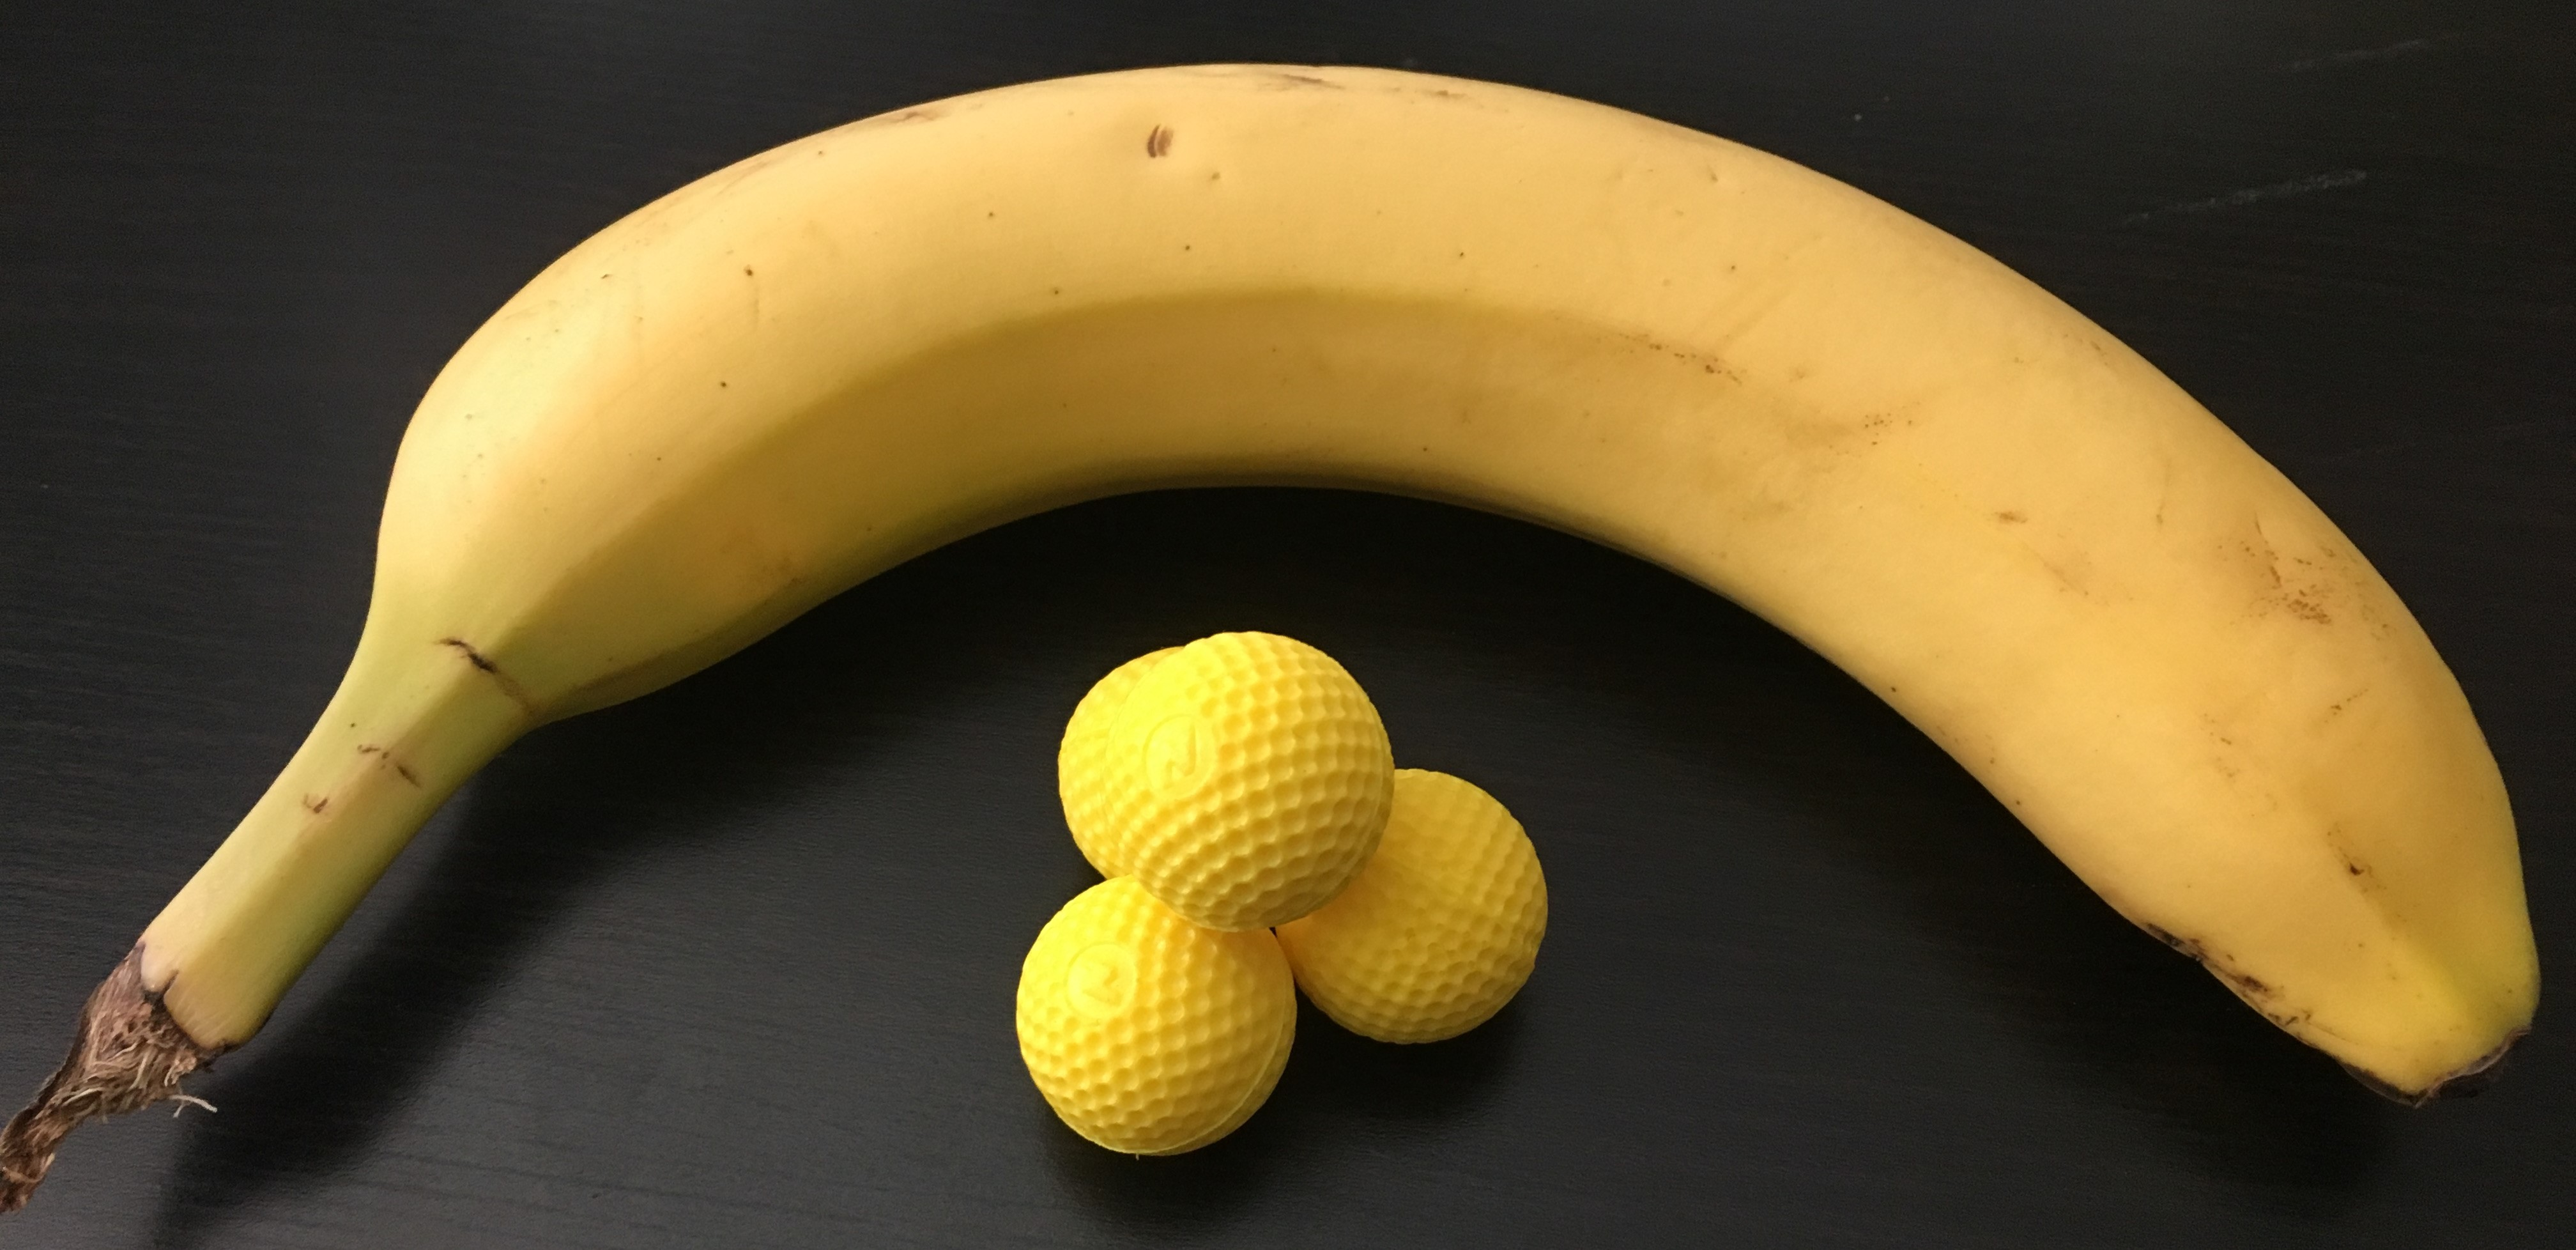
\includegraphics[width=6in, height=3.85in, keepaspectratio]{figures/nerf_rival_balls.jpg}
	\caption{Nerf Rival Balls with Banana for Scale}	\label{fig:nerf_rival_balls}
\end{figure}
